\subsection{Shielding}

Effective shielding is of great interest to reduce EMI of electronic systems. A figure of merit for shielding capabilities of a material is the electromagnetic shielding effectiveness (SE), given in \autoref{eqn:se_elec_fields} \cite{10518640}. $E_\mathrm{i}$ is the incident electric field, while $E_\mathrm{t}$ is the transmitted electric field, also depicted in \autoref{fig:shielding_material_diagram}. It depends on the thickness and shape of the material, and its electric and magnetic properties. Additionally, the TEM cell contributes to the SE values.

% Should I add wave reflections formula?

\begin{equation}
    SE_{\mathrm{dB}}=20\log{(\frac{E_\mathrm{i}}{E_\mathrm{t}})}
    \label{eqn:se_elec_fields}
\end{equation}

\begin{figure}[h]
    \centering
    \includegraphics[width=0.35\linewidth]{images/shielding_material_diagram.png}
    \caption{Incident, reflected and transmitted electric fields due to interaction with shielding material}
    \label{fig:shielding_material_diagram}
\end{figure}

% (Note: Higher order modes may be able to propagate in the TEM cell, as the refraction of the shielding material follows to excitation of these modes.)

An electromagnetic wave may undergo several reflections inside the shielding material, with each reflection adding up to the total reflected, absorbed and transmitted waves. The total shielding effectiveness is therefore determined by \autoref{eqn:se_rereflections}, according to Schelkunoff. $A_{\mathrm{dB}}$ represents the absorption losses traveling through the shield, $R_{\mathrm{dB}}$ the reflection losses, and $B_{\mathrm{dB}}$ is the correction factor for the multiple reflections inside the shield \cite{10518640}.

\begin{equation}
    SE_{\mathrm{dB}}=R_{\mathrm{dB}}+A_{\mathrm{dB}}+B_{\mathrm{dB}}
    \label{eqn:se_rereflections}
\end{equation}

Calculate with S-params $S_{11}$ and $S_{21}$: A, R and T.  

This approach to shielding with internal re-reflections in the shielding material was derived by Schelkunoff. 
\url{https://www.ieee.li/pdf/viewgraphs/fundamentals_electromagnetic_shield.pdf}

The reflections occur due to the change in wave impedance. They are described through a reflection coefficient $R$. Additionally, it is common to normalize the wave impedance $Z$ to the free-space wave impedance $Z_0$. At the interface from free-space to a shielding material, this leads to \autoref{eqn:reflection_coefficient_plane_dielectric} \cite{Collin_2015}. 

\begin{equation}
    R=\frac{Z-1}{Z+1}
    \label{eqn:reflection_coefficient_plane_dielectric}
\end{equation}

\begin{equation}
    Z=\frac{1}{Z_0}\sqrt{\frac{\mathrm{i}\omega\mu}{\sigma+\mathrm{i}\omega\epsilon}}
    \label{eqn:rel_wave_imp}
\end{equation}

The reflection coefficient can be converted into dB, leading to $R_\mathrm{dB}$. Any additional reflection happen due to re-reflections inside the shielding material, described by $B_\mathrm{dB}$. The rest of the energy must either be absorbed, described by $A_\mathrm{dB}$ or transmitted, shown by $T_\mathrm{dB}$. 

\todo{p. 309 Classical Electrodynamics (John David Jackson) describe shielding material by dipole moments}

The wave number $k$ in lossy media is described in a real an imaginary parts as in \autoref{eqn:wave_number}. The imaginary part $\alpha$ is the attenuation or absorption coefficient. It describes the reduction of the intensity of the wave, which occurs with $\mathrm{e}^{-\alpha x}$, where x is the coordinate direction of propagation. The real part $\beta=\frac{2\pi}{\lambda}$ is the phase constant \cite{Jackson}.

\todo{Formula $\alpha$? Needed?}

\begin{equation}
    k = \beta + \mathrm{i}\frac{\alpha}{2}
    \label{eqn:wave_number}
\end{equation}
\begin{equation}
    \mathbf{E} = \mathbf{e}\cdot \mathrm{e}^{\mathrm{i}kx}
\end{equation}

\todo{S-parameters should enable derivation of $\alpha$. Due to normal incident wave of TEM, no angle needed to consider.}

% Quick mathematical formulation of how to calculate reflected waves?

\todo{Basics: Balanis 2012 page 68?}

When the molecules in a material are exposed to electric fields, they will polarize, described by their permittivity $\epsilon$. When exposed to a magnetic field, the spinning of their electrons in the atoms align with the magnetic field, described by the permeability $\mu$ of the material. When the fields alternate over time, the molecules will always move and align according to them. This is essentially a movement of charges, and therefore described by a conductivity $\sigma$. The energy lost in this process is dissipated as heat \cite{Balanis_2012}.

The electric field will push charges in polarizable molecules apart. This separation of charges may be described as a electric dipole, depending on the separation distance and the charge. Under alternating electric fields, the moving of charges will contribute to $\sigma$. This phenomenon is called dielectric hysteresis. \autoref{eqn:loss_tangent_permittivity} quantifies it by a loss tangent $\tan\delta_e$ \cite{Balanis_2012}. There, $\sigma_s$ is the static conductivity, meaning the conductivity of the material for static fields. The complex part of the permittivity $\epsilon''$ describes the lossy part of the dielectric material, specifically relevant for the alternating fields case. The real part of the permittivity is lossless and is noted by $\epsilon'$. The overall complex permittivity is therefore $\epsilon=\epsilon'+\mathrm{i}\epsilon''$.
\todo{Some way to describe coupling of shielding material to TEM cell?}

\begin{equation}
    \tan\delta_e = \frac{\sigma_s}{\omega\epsilon'}+\frac{\epsilon''}{\epsilon'}
    \label{eqn:loss_tangent_permittivity}
\end{equation}

The loss tangent therefore $\tan\delta_e$ relates the conductivity of a material to the real permittivity. A dielectric with low losses has a much larger displacement current than conduction current density ($\tan\delta_e \ll 1$). The opposite is true for a good conductor ($\tan\delta_e \gg 1$) \cite{Balanis_2012}.

The loss tangent $\tan\delta_e$ is a function of frequency, however, it is often not stated as such. Therefore, the loss tangent of FR4, for example, is given as $\tan\delta_e=0.02$ for frequencies up to 1\,GHz. For higher frequencies, the molecules may have resonance frequencies, where they influence more strongly the overall conductance and consequently increase the imaginary part of the permittivity $\epsilon''$.

There are also magnetically lossy materials, which is introduced by a complex permeability $\mu=\mu'+\mathrm{i}\mu''$. Analog to the dielectric case, the permeability can also be described by a loss tangent $\tan{\delta_m}$ as shown in \autoref{eqn:magnetic_loss_tangent}. However, the loss tangent is very low for the majority of materials and will be neglected. Ferrites are an exception, which are commonly used to dampen high frequency signals \cite{Balanis_2012}.

\begin{equation}
    \tan{\delta_m}=\frac{\mu''}{\mu'}
    \label{eqn:magnetic_loss_tangent}
\end{equation}


\todo{describe $\alpha$ and $\delta$ for absorption. Then reflections with $\epsilon$ and $\mu$}

Electric fields dominate in the near-field region of electric dipoles. To shield them, high permittivity and high conductivity materials, ideally with a high loss tangent $\tan\delta_e$ shall be used. On the other hand, magnetic fields dominate in the near-field region of magnetic dipoles. For shielding them, high permittivity and high conductivity materials, again with a high loss tangent $\tan\delta_m$ shall be used.\todo{source}

\subsubsection{ASTM ES7-83 Method}

The ASTM ES7-83 method is used to determine the shielding effectiveness of shielding materials. The shielding material is inserted into a coaxial TEM cell around the septum. Ideally, they form a continuous connection \cite{MORARI_BĂLAN_2015}. 

In this method, two measurements are performed with an oscilloscope attached to the output of the TEM cell. In the first, an empty TEM cell is excited and a reference output voltage $U_\mathrm{ref}$ is measured. In the second, the TEM cell is loaded with the shielding material, and the output voltage $U_\mathrm{load}$ is again noted. The measurement values are then used in \autoref{eqn:SE_voltages} to derive the shielding effectiveness $SE_\mathrm{dB}$ \cite{MORARI_BĂLAN_2015}.

\begin{equation}
    SE_\mathrm{dB}=20\cdot\log{\left(\frac{U_\mathrm{ref}}{U_\mathrm{load}}\right)}
    \label{eqn:SE_voltages}
\end{equation}

In the case of simulating the problem, such a procedure may be used, too. It is more convenient, then, to defined a reference output power $P_\mathrm{ref}$ for an unloaded TEM cell, and a output power for the loaded case $P_\mathrm{load}$. This leads to the similar \autoref{eqn:SE_power}.

\begin{equation}
    SE_\mathrm{dB}=10\cdot\log{\left( \frac{P_\mathrm{ref}}{P_\mathrm{load}} \right)}
    \label{eqn:SE_power}
\end{equation}

Additionally, a rectangular TEM cell is used for this method, instead of the commonly used cylindrical version. \autoref{fig:form_of_shielding_material} shows the cross section of this shielding material, which is inserted into the TEM cell. In \autoref{fig:ASTM ES7-83} the shielding material can be seen wrapped around the septum. 

\begin{figure}[h]
    \centering
    \begin{subfigure}[h]{0.49\textwidth}
        \centering
        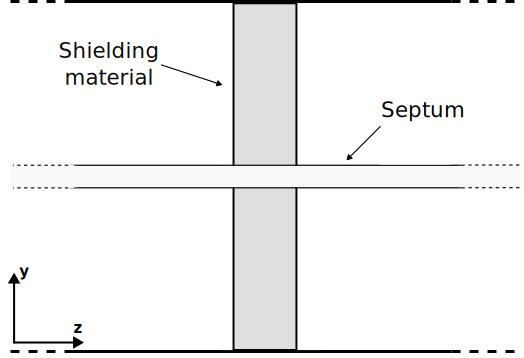
\includegraphics[width=\textwidth]{content//10_theory//img/ASTM ES7-83.png}
        \caption{Shielding material in TEM cell}
        \label{fig:ASTM ES7-83}
    \end{subfigure}%
    \hfill
    \begin{subfigure}[h]{0.49\textwidth}
        \centering
        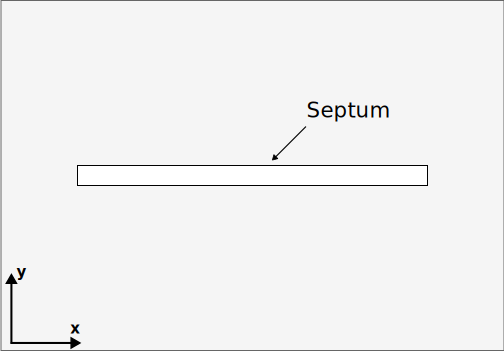
\includegraphics[width=\textwidth]{content//10_theory/img/form_of_shielding_material.png}
        \caption{Shape of the shielding material}
        \label{fig:form_of_shielding_material}
    \end{subfigure}
    \label{fig:subfigures}
\end{figure}

Then, the S-parameters derived in the simulations are used to get to the output powers $P_\mathrm{ref}$ and $P_\mathrm{load}$. By exciting the TEM cell with a power of 1\,W, the reference power $P_\mathrm{ref}=1\,\mathrm{W}$. The measured power is then derived through \autoref{eqn:load_power}.

\begin{equation}
    P_\mathrm{load}=P_\mathrm{ref}\cdot10^{|S_\mathrm{12}|/10}
    \label{eqn:load_power}
\end{equation}


\todo{Describe Method. Then follows dual TEM cells}

\subsubsection{Dual TEM cell}

The shielding effectiveness of a material may also be determined using two TEM cells, which are stacked upon each other, as shown in \autoref{fig:dual_tem_cell}. They are connected through an aperture, which can be filled with the shielding material. One TEM cell is excited, and therefore acts as a driving cell. It transmits power through the aperture. It is measured at the second TEM cell, which acts as a receiver. The dual TEM cell simulates near-field conditions, opposed to the far-field conditions simulated by the simple TEM cell \cite{MORARI_BĂLAN_2015}. This is important when using the shielding material to shield an antenna's radiation by placing the material directly next to it.

The electrically small aperture may be described by an electric and a magnetic dipole moment\todo{must it be electrically small?}. Their magnitude is related to the electric and magnetic coupling between the TEM cells over the aperture. Therefore, the electric and magnetic coupling can be determined separately by adding or subtracting the output powers of the receiving TEM cell \cite{MORARI_BĂLAN_2015, 4091811}. Consequently, a electric shielding effectiveness $SE_\mathrm{dB}^\mathrm{e}$ can be calculated with \autoref{eqn:se_dual_cell_e}, and a magnetic shielding effectiveness $SE_\mathrm{dB}^\mathrm{m}$ with \autoref{eqn:se_dual_cell_m}. If a material, for example, permits energy transfer because of magnetic dipoles in it, then a measurement with lower $SE_\mathrm{dB}^\mathrm{m}$ than $SE_\mathrm{dB}^\mathrm{e}$ is to be expected \cite{4091811}.


\begin{subequations}
    \begin{equation}
        SE_\mathrm{dB}^\mathrm{e}=10\log{\left( \frac{P_\mathrm{ref, sum}}{P_\mathrm{load,sum}} \right)}
        \label{eqn:se_dual_cell_e}
    \end{equation}
    \begin{equation}
        SE_\mathrm{dB}^\mathrm{m}=10\log{\left( \frac{P_\mathrm{ref, diff}}{P_\mathrm{load,diff}} \right)}
        \label{eqn:se_dual_cell_m}
    \end{equation}
\end{subequations}

Because the normalized electric field at the aperture will be of TEM mode, only the component normal to the aperture in z-direction has to be considered. Just as in the case of dipole representation, the Lorentz Reciprocity theorem may be applied to find the fields in the TEM cell. Because both the fields at the output and in the aperture are of TEM mode, only the E-field at the output may be considered. 

Since the aperture is electrically small, the field quantities may be assumed to be constant over it. This makes it possible to represent the energy transfer by dipole moments. \todo{Polarization of the material. Small aperture theory.}

\begin{figure}[h]
    \centering
    \includegraphics[width=0.75\linewidth]{content//10_theory//img/dual_tem_cell.png}
    \caption{Dual TEM cell with aperture}
    \label{fig:dual_tem_cell}
\end{figure}

